%&preformat-disser
\RequirePackage[l2tabu,orthodox]{nag} % Раскомментировав, можно в логе получать рекомендации относительно правильного использования пакетов и предупреждения об устаревших и нерекомендуемых пакетах
% Формат А4, 14pt (ГОСТ Р 7.0.11-2011, 5.3.6)
\documentclass[a4paper,14pt,oneside,openany]{memoir}


\input{common/setup}            % общие настройки шаблона
%%% Проверка используемого TeX-движка %%%
\RequirePackage{ifxetex, ifluatex}
\newif\ifxetexorluatex   % определяем новый условный оператор (http://tex.stackexchange.com/a/47579)
\ifxetex
    \xetexorluatextrue
\else
    \ifluatex
        \xetexorluatextrue
    \else
        \xetexorluatexfalse
    \fi
\fi

\newif\ifsynopsis           % Условие, проверяющее, что документ --- автореферат

\RequirePackage{etoolbox}[2015/08/02]               % Для продвинутой проверки разных условий
\providebool{presentation}

\usepackage{cite}
\usepackage[resetlabels]{multibib}
\newcites{author}{References}

%%% Поля и разметка страницы %%%
\usepackage{pdflscape}                              % Для включения альбомных страниц
\usepackage{geometry}                               % Для последующего задания полей

%%% Математические пакеты %%%
\usepackage{amsthm,amsmath,amscd}   % Математические дополнения от AMS
\usepackage{amsfonts,amssymb}       % Математические дополнения от AMS
\usepackage{mathtools}              % Добавляет окружение multlined

%%%% Установки для размера шрифта 14 pt %%%%
%% Формирование переменных и констант для сравнения (один раз для всех подключаемых файлов)%%
%% должно располагаться до вызова пакета fontspec или polyglossia, потому что они сбивают его работу
\newlength{\curtextsize}
\newlength{\bigtextsize}
\setlength{\bigtextsize}{13.9pt}

\makeatletter
%\show\f@size                                       % неплохо для отслеживания, но вызывает стопорение процесса, если документ компилируется без команды  -interaction=nonstopmode
\setlength{\curtextsize}{\f@size pt}
\makeatother

%%% Кодировки и шрифты %%%
\ifxetexorluatex
    \usepackage{polyglossia}[2014/05/21]            % Поддержка многоязычности (fontspec подгружается автоматически)
\else
   %%% Решение проблемы копирования текста в буфер кракозябрами
    \ifnumequal{\value{usealtfont}}{0}{}{
        \input glyphtounicode.tex
        \input glyphtounicode-cmr.tex %from pdfx package
        \pdfgentounicode=1
    }
    \usepackage{cmap}                               % Улучшенный поиск русских слов в полученном pdf-файле
    \ifnumequal{\value{usealtfont}}{2}{}{
        \defaulthyphenchar=127                      % Если стоит до fontenc, то переносы не впишутся в выделяемый текст при копировании его в буфер обмена
    }
    \usepackage{textcomp}
    \usepackage[T1,T2A]{fontenc}                    % Поддержка русских букв
    \ifnumequal{\value{usealtfont}}{1}{% Используется pscyr, при наличии
        \IfFileExists{pscyr.sty}{\usepackage{pscyr}}{}  % Подключение pscyr
    }{}
    \usepackage[utf8]{inputenc}[2014/04/30]         % Кодировка utf8
    \usepackage[english, russian]{babel}[2014/03/24]% Языки: русский, английский
    \ifnumequal{\value{usealtfont}}{2}{
        % http://dxdy.ru/post1238763.html#p1238763
        \usepackage[scaled=0.960]{XCharter}[2017/12/19] % Подключение русифицированных шрифтов XCharter
        \usepackage[charter, vvarbb, scaled=1.048]{newtxmath}[2017/12/14]
        \setDisplayskipStretch{-0.078}
    }{}
\fi

%%% Оформление абзацев %%%
\usepackage{indentfirst}                            % Красная строка

%%% Цвета %%%
\ifpresentation
\else
    \usepackage[dvipsnames, table, hyperref]{xcolor} % Совместимо с tikz
\fi

%%% Таблицы %%%
\usepackage{longtable,ltcaption}                    % Длинные таблицы
\usepackage{multirow,makecell}                      % Улучшенное форматирование таблиц

%%% Общее форматирование
\usepackage{soulutf8}                               % Поддержка переносоустойчивых подчёркиваний и зачёркиваний
\usepackage{icomma}                                 % Запятая в десятичных дробях

%%% Оптимизация расстановки переносов и длины последней строки абзаца
\ifluatex
    \ifnumequal{\value{draft}}{1}{% Черновик
        \usepackage[hyphenation, lastparline, nosingleletter, homeoarchy,
        rivers, draft]{impnattypo}
    }{% Чистовик
        \usepackage[hyphenation, lastparline, nosingleletter]{impnattypo}
    }
\else
    \usepackage[hyphenation, lastparline]{impnattypo}
\fi

%%% Гиперссылки %%%
\usepackage{hyperref}[2012/11/06]

%%% Изображения %%%
\usepackage{graphicx}[2014/04/25]                   % Подключаем пакет работы с графикой

%%% Счётчики %%%
\usepackage[figure,table]{totalcount}               % Счётчик рисунков и таблиц
\usepackage{totcount}                               % Пакет создания счётчиков на основе последнего номера подсчитываемого элемента (может требовать дважды компилировать документ)
\usepackage{totpages}                               % Счётчик страниц, совместимый с hyperref (ссылается на номер последней страницы). Желательно ставить последним пакетом в преамбуле

%%% Продвинутое управление групповыми ссылками (пока только формулами) %%%
\ifpresentation
\else
    \ifxetexorluatex
        \usepackage{cleveref}                           % cleveref корректно считывает язык из настроек polyglossia
    \else
        \usepackage[russian]{cleveref}                  % cleveref имеет сложности со считыванием языка из babel. Такое решение русификации вывода выбрано вместо определения в documentclass из опасности что-то лишнее передать во все остальные пакеты, включая библиографию.
    \fi
    \creflabelformat{equation}{#2#1#3}                  % Формат по умолчанию ставил круглые скобки вокруг каждого номера ссылки, теперь просто номера ссылок без какого-либо дополнительного оформления
    \crefrangelabelformat{equation}{#3#1#4\cyrdash#5#2#6}   % Интервалы в русском языке принято делать через тире, если иное не оговорено
\fi

\ifnumequal{\value{draft}}{1}{% Черновик
    \usepackage[firstpage]{draftwatermark}
    \SetWatermarkText{DRAFT}
    \SetWatermarkFontSize{14pt}
    \SetWatermarkScale{15}
    \SetWatermarkAngle{45}
}{}

%%% Исправление положения якорей подписей (под)рисунков %%%
% Без hypcap и патча, при клике по ссылке на подрисунок, просмотрщик pdf прыгает "к подписи" а не "к рисунку".
% Подробнее: https://github.com/AndreyAkinshin/Russian-Phd-LaTeX-Dissertation-Template/issues/238
% (!) Даже с патчем, если мешать в одной фиге разные типы подфиг (subbottom и subcaption) - ссылки всё равно будут работать неправильно  (см. https://www.overleaf.com/read/czmbmmtnqrrg ).
\ifpresentation
\else
    \usepackage[all]{hypcap}

    \makeatletter
    \ltx@ifclasslater{memoir}{2018/12/13}{
        % Предполагается, что в следующей версии класс будет исправлен
        \typeout{Assuming this version of memoir is free from the jumping-to-caption bug.}
    }{
        \RequirePackage{xpatch}

        \newcommand\mem@step@subcounter{\refstepcounter{sub\@captype}\@contkeep}

        \xpatchcmd{\@memsubbody}%
        {\refstepcounter{sub\@captype}\@contkeep}% search pattern
        {}% replacement
        {\typeout{@memsubbody is patched}}%
        {\typeout{@memsubbody is NOT patched}}%

        \xpatchcmd{\@memcontsubbody}%
        {\refstepcounter{sub\@captype}\@contkeep}% pattern
        {}% replacement
        {\typeout{@memcontsubbody is patched}}%
        {\typeout{@memcontsubbody is NOT patched}}%

        \xpatchcmd{\@memsubfloat}%
        {\vbox\bgroup}% search pattern
        {\vbox\bgroup\mem@step@subcounter}% replacement
        {\typeout{@memsubfloat patch is ok}}%
        {\typeout{@memsubfloat patch is NOT ok}}%

        \xpatchcmd{\subcaption}%
        {\refstepcounter{sub\@captype}}% search pattern
        {\H@refstepcounter{sub\@captype}}% replacement
        {\typeout{subcaption second patch is ok}}%
        {\typeout{subcaption second patch is NOT ok}}%
    }
    \makeatother
\fi

%%% Цитата, не приводимая в автореферате:
% возможно, актуальна только для biblatex
%\newcommand{\citeinsynopsis}[1]{\ifsynopsis\else ~\cite{#1} \fi}
         % Пакеты общие для диссертации и автореферата
\synopsisfalse                      % Этот документ --- не автореферат
\input{Dissertation/dispackages}    % Пакеты для диссертации
\input{Dissertation/userpackages}   % Пакеты для специфических пользовательских задач

\input{Dissertation/setup}      % Упрощённые настройки шаблона

% Новые переменные, которые могут использоваться во всём проекте
% ГОСТ 7.0.11-2011
% 9.2 Оформление текста автореферата диссертации
% 9.2.1 Общая характеристика работы включает в себя следующие основные структурные
% элементы:
% актуальность темы исследования;
\newcommand{\actualityTXT}{Актуальность темы.}
% степень ее разработанности;
\newcommand{\progressTXT}{Степень разработанности темы.}
% цели и задачи;
\newcommand{\aimTXT}{Целью}
\newcommand{\tasksTXT}{задачи}
% научную новизну;
\newcommand{\noveltyTXT}{Научная новизна:}
% теоретическую и практическую значимость работы;
%\newcommand{\influenceTXT}{Теоретическая и практическая значимость}
% или чаще используют просто
\newcommand{\influenceTXT}{Практическая значимость:}
% методологию и методы исследования;
\newcommand{\methodsTXT}{Методология и методы исследования.}
% положения, выносимые на защиту;
\newcommand{\defpositionsTXT}{Положения, выносимые на публичное представление:}
% степень достоверности и апробацию результатов.
\newcommand{\reliabilityTXT}{Работоспособность}
\newcommand{\probationTXT}{Апробация работы.}

\newcommand{\contributionTXT}{Личный вклад.}
\newcommand{\publicationsTXT}{Публикации.}


%%% Заголовки библиографии:

% для автореферата:
\newcommand{\bibtitleauthor}{Публикации автора по теме диссертации}

% для стиля библиографии `\insertbiblioauthorgrouped`
\newcommand{\bibtitleauthorvak}{В изданиях из списка ВАК РФ}
\newcommand{\bibtitleauthorscopus}{В изданиях, входящих в международную базу цитирования Scopus}
\newcommand{\bibtitleauthorwos}{В изданиях, входящих в международную базу цитирования Web of Science}
\newcommand{\bibtitleauthorother}{В прочих изданиях}
\newcommand{\bibtitleauthorconf}{В сборниках трудов конференций}

% для стиля библиографии `\insertbiblioauthorimportant`:
\newcommand{\bibtitleauthorimportant}{Наиболее значимые \protect\MakeLowercase\bibtitleauthor}

% для списка литературы в диссертации и списка чужих работ в автореферате:
\newcommand{\bibtitlefull}{Список литературы} % (ГОСТ Р 7.0.11-2011, 4)
         % Новые переменные, для всего проекта

%%% Основные сведения %%%
\newcommand{\thesisAuthorLastName}{Доронина}
\newcommand{\thesisAuthorOtherNames}{Ольга Александровна}
\newcommand{\thesisAuthorInitials}{О.\,А.}
\newcommand{\thesisAuthor}             % Диссертация, ФИО автора
{%
    \texorpdfstring{% \texorpdfstring takes two arguments and uses the first for (La)TeX and the second for pdf
        \thesisAuthorLastName~\thesisAuthorOtherNames% так будет отображаться на титульном листе или в тексте, где будет использоваться переменная
    }{%
        \thesisAuthorLastName, \thesisAuthorOtherNames% эта запись для свойств pdf-файла. В таком виде, если pdf будет обработан программами для сбора библиографических сведений, будет правильно представлена фамилия.
    }
}
\newcommand{\thesisAuthorShort}        % Диссертация, ФИО автора инициалами
{\thesisAuthorInitials~\thesisAuthorLastName}
%\newcommand{\thesisUdk}                % Диссертация, УДК
%{\todo{xxx.xxx}}
\newcommand{\thesisTitle}              % Диссертация, название
{\todo{Длинное название диссертационной работы, состоящее из~достаточно большого
количества слов, совсем длинное длинное длинное длинное название, из~которого
простому обывателю знакомы, в~лучшем случае, лишь отдельные слова}}
\newcommand{\thesisSpecialtyNumber}    % Диссертация, специальность, номер
{09.06.01}
\newcommand{\thesisSpecialtyTitle}     % Диссертация, специальность, название (название взято с сайта ВАК для примера)
{Информатика и вычислительная техника}
%% \newcommand{\thesisSpecialtyTwoNumber} % Диссертация, вторая специальность, номер
%% {\todo{XX.XX.XX}}
\newcommand{\thesisSpecialtyTwoTitle}  % Диссертация, вторая специальность, название
{{Математическое моделирование, численные методы и комплексы программ}}
\newcommand{\thesisDegree}             % Диссертация, ученая степень
{\todo{кандидата физико-математических наук}}
\newcommand{\thesisDegreeShort}        % Диссертация, ученая степень, краткая запись
{\todo{канд. физ.-мат. наук}}
\newcommand{\thesisCity}               % Диссертация, город написания диссертации
{Москва}
\newcommand{\thesisYear}               % Диссертация, год написания диссертации
{2019}
\newcommand{\thesisOrganization}       % Диссертация, организация
{Федеральное государственное автономное образовательное учреждение высшего
		образования <<Московский физико-технический институт (государственный университет)>>}
\newcommand{\thesisOrganizationShort}  % Диссертация, краткое название организации для доклада
{МФТИ(ГУ)}

\newcommand{\thesisInOrganization}     % Диссертация, организация в предложном падеже: Работа выполнена в ...
{\todo{учреждении с~длинным длинным длинным длинным названием, в~котором
выполнялась данная диссертационная работа}}

%% \newcommand{\supervisorDead}{}           % Рисовать рамку вокруг фамилии
\newcommand{\supervisorFio}              % Научный руководитель, ФИО
{Четверушкин Борис Николаевич}
\newcommand{\supervisorRegalia}          % Научный руководитель, регалии
{д.ф.-м.н., профессор, академик РАН}
\newcommand{\supervisorFioShort}         % Научный руководитель, ФИО
{Б.\,Н.~Четверушкин}
\newcommand{\supervisorRegaliaShort}     % Научный руководитель, регалии
{д.ф.-м.н., профессор, академик РАН}

%% \newcommand{\supervisorTwoDead}{}        % Рисовать рамку вокруг фамилии
%% \newcommand{\supervisorTwoFio}           % Второй научный руководитель, ФИО
%% {\todo{Фамилия Имя Отчество}}
%% \newcommand{\supervisorTwoRegalia}       % Второй научный руководитель, регалии
%% {\todo{уч. степень, уч. звание}}
%% \newcommand{\supervisorTwoFioShort}      % Второй научный руководитель, ФИО
%% {\todo{И.\,О.~Фамилия}}
%% \newcommand{\supervisorTwoRegaliaShort}  % Второй научный руководитель, регалии
%% {\todo{уч.~ст.,~уч.~зв.}}

\newcommand{\opponentOneFio}           % Оппонент 1, ФИО
{\todo{Фамилия Имя Отчество}}
\newcommand{\opponentOneRegalia}       % Оппонент 1, регалии
{\todo{доктор физико-математических наук, профессор}}
\newcommand{\opponentOneJobPlace}      % Оппонент 1, место работы
{\todo{Не очень длинное название для места работы}}
\newcommand{\opponentOneJobPost}       % Оппонент 1, должность
{\todo{старший научный сотрудник}}

\newcommand{\opponentTwoFio}           % Оппонент 2, ФИО
{\todo{Фамилия Имя Отчество}}
\newcommand{\opponentTwoRegalia}       % Оппонент 2, регалии
{\todo{кандидат физико-математических наук}}
\newcommand{\opponentTwoJobPlace}      % Оппонент 2, место работы
{\todo{Основное место работы c длинным длинным длинным длинным названием}}
\newcommand{\opponentTwoJobPost}       % Оппонент 2, должность
{\todo{старший научный сотрудник}}

%% \newcommand{\opponentThreeFio}         % Оппонент 3, ФИО
%% {\todo{Фамилия Имя Отчество}}
%% \newcommand{\opponentThreeRegalia}     % Оппонент 3, регалии
%% {\todo{кандидат физико-математических наук}}
%% \newcommand{\opponentThreeJobPlace}    % Оппонент 3, место работы
%% {\todo{Основное место работы c длинным длинным длинным длинным названием}}
%% \newcommand{\opponentThreeJobPost}     % Оппонент 3, должность
%% {\todo{старший научный сотрудник}}

\newcommand{\leadingOrganizationTitle} % Ведущая организация, дополнительные строки. Удалить, чтобы не отображать в автореферате
{\todo{Федеральное государственное бюджетное образовательное учреждение высшего
профессионального образования с~длинным длинным длинным длинным названием}}

\newcommand{\defenseDate}              % Защита, дата
{\todo{DD mmmmmmmm YYYY~г.~в~XX часов}}
\newcommand{\defenseCouncilNumber}     % Защита, номер диссертационного совета
{\todo{Д\,123.456.78}}
\newcommand{\defenseCouncilTitle}      % Защита, учреждение диссертационного совета
{\todo{Название учреждения}}
\newcommand{\defenseCouncilAddress}    % Защита, адрес учреждение диссертационного совета
{\todo{Адрес}}
\newcommand{\defenseCouncilPhone}      % Телефон для справок
{\todo{+7~(0000)~00-00-00}}

\newcommand{\defenseSecretaryFio}      % Секретарь диссертационного совета, ФИО
{\todo{Фамилия Имя Отчество}}
\newcommand{\defenseSecretaryRegalia}  % Секретарь диссертационного совета, регалии
{\todo{д-р~физ.-мат. наук}}            % Для сокращений есть ГОСТы, например: ГОСТ Р 7.0.12-2011 + http://base.garant.ru/179724/#block_30000

\newcommand{\synopsisLibrary}          % Автореферат, название библиотеки
{\todo{Название библиотеки}}
\newcommand{\synopsisDate}             % Автореферат, дата рассылки
{\todo{DD mmmmmmmm YYYY года}}

% To avoid conflict with beamer class use \providecommand
\providecommand{\keywords}%            % Ключевые слова для метаданных PDF диссертации и автореферата
{}
             % Основные сведения
\input{common/fonts}            % Определение шрифтов (частичное)
\input{common/styles}           % Стили общие для диссертации и автореферата
\input{Dissertation/disstyles}  % Стили для диссертации
\input{Dissertation/userstyles} % Стили для специфических пользовательских задач

%%% Библиография. Выбор движка для реализации %%%
\ifnumequal{\value{bibliosel}}{0}{%
    \input{biblio/predefined}   % Встроенная реализация с загрузкой файла через движок bibtex8
}{
    \input{biblio/biblatex}     % Реализация пакетом biblatex через движок biber
}

% Вывести информацию о выбранных опциях в лог сборки
\typeout{Selected options:}
\typeout{Draft mode: \arabic{draft}}
\typeout{Font: \arabic{fontfamily}}
\typeout{AltFont: \arabic{usealtfont}}
\typeout{Bibliography backend : \arabic{bibliosel}}
\typeout{Precompile images : \arabic{imgprecompile}}

%%% Управление компиляцией отдельных частей диссертации %%%
% Необходимо сначала иметь полностью скомпилированный документ, чтобы все
% промежуточные файлы были в наличии
% Затем, для вывода отдельных частей можно воспользоваться командой \includeonly
% Ниже примеры использования команды:
%
%\includeonly{Dissertation/part2}
%\includeonly{Dissertation/contents,Dissertation/appendix,Dissertation/conclusion}
%
% Если все команды закомментированы, то документ будет выведен в PDF файл полностью

\begin{document}

\input{common/renames}                 % Переопределение именований

%%% Структура диссертации (ГОСТ Р 7.0.11-2011, 4)
% Титульный лист (ГОСТ Р 7.0.11-2001, 5.1)
\thispagestyle{empty}
\begin{center}
\thesisOrganization
\end{center}
%



\vspace{0pt plus4fill} %число перед fill = кратность относительно некоторого расстояния fill, кусками которого заполнены пустые места
%

{\small
	\noindent\textbf{Направление подготовки:} \thesisSpecialtyNumber\, \thesisSpecialtyTitle
}

\ifdefined\thesisSpecialtyTwoNumber
{\small
	\noindent\textbf{Направленность (профиль) подготовки:} \thesisSpecialtyTwoNumber\, \thesisSpecialtyTwoTitle
}
\fi

\ifdefined\educationForm
{\small
	\noindent\textbf{Форма обучения:} \educationForm
}
\fi
\vspace{0pt plus6fill} %число перед fill = кратность относительно некоторого расстояния fill, кусками которого заполнены пустые места
\begin{center}
{\large \thesisAuthor}
\end{center}
%
\vspace{0pt plus1fill} %число перед fill = кратность относительно некоторого расстояния fill, кусками которого заполнены пустые места
\begin{center}
\textbf {\large %\MakeUppercase
\thesisTitle}

\vspace{0pt plus2fill} %число перед fill = кратность относительно некоторого расстояния fill, кусками которого заполнены пустые места




\vspace{0pt plus2fill} %число перед fill = кратность относительно некоторого расстояния fill, кусками которого заполнены пустые места
Диссертация на соискание учёной степени

\thesisDegree
\end{center}
%
\vspace{0pt plus4fill} %число перед fill = кратность относительно некоторого расстояния fill, кусками которого заполнены пустые места
\begin{flushright}
\ifdefined\supervisorTwoFio
Научные руководители:

\supervisorRegalia

\ifdefined\supervisorDead
\framebox{\supervisorFio}
\else
\supervisorFio
\fi

\supervisorTwoRegalia

\ifdefined\supervisorTwoDead
\framebox{\supervisorTwoFio}
\else
\supervisorFio
\fi
\else
Научный руководитель:

\supervisorRegalia

\ifdefined\supervisorDead
\framebox{\supervisorFio}
\else
\supervisorFio
\fi
\fi

\end{flushright}
%
\vspace{0pt plus4fill} %число перед fill = кратность относительно некоторого расстояния fill, кусками которого заполнены пустые места
{\centering\thesisCity\ "--- \thesisYear\par}
           % Титульный лист
\include{Dissertation/contents}        % Оглавление
\chapter*{Введение}                         % Заголовок
\addcontentsline{toc}{chapter}{Введение}    % Добавляем его в оглавление
	Одной из наиболее сложных задач вычислительной газовой динамики и аэродинамики, в частности, является математическое моделирование течений вокруг движущихся тел. Численное предсказание возникающих таким образом сложных взаимосвязанных газодинамических явлений может внести существенный вклад в решение большого числа фундаментальных проблем в аэродинамике систем перемещающихся тел и/или движущихся элементов одного тела. К таким задачам можно отнести исследование аэродинамических и акустических свойств крыла самолёта с механизацией, включая выдвигающиеся или задвигающиеся закрылки и предкрылки; влияние на аэродинамику и акустику открывающихся технологических отсеков и выдвигаемых частей, например, при выпускании шасси самолёта; моделирование траектории сбрасываемых грузов и ряд других проблем. В таких задачах могут присутствовать два типа тел, движущихся относительно друг друга. Первый тип – это основное, родительское, тело, второй – тело или тела, совершающие, вообще говоря, достаточно сложные движения относительно основного тела. В такой ситуации трудно, а порою даже невозможно, использовать традиционный подход к описанию обтекаемого объекта граничными узлами или граничными элементами расчётной сетки. Такой подход логично применить только к покоящемуся родительскому телу, в системе расчёта которого моделировать передвижения остальных, более мелких, объектов. Для описания движущихся тел в качестве наиболее удобного подхода все большее распространение приобретают методы погруженных границ (в англоязычной научной литературе – Immersed Boundary Conditions или IBC метод)~\cite{mittal2005immersed, boiron2009high, brown2014characteristic}.

	Методы погруженных границ составляют целый класс методов, позволяющих обес-печить выполнение граничных условий на поверхности обтекаемых тел в процессе численного расчета без описания ее геометрии сеточными узлами. Это означает, что может быть использована «сплошная» расчетная сетка, покрывающая всю область определения зада-чи, включая препятствие. Взаимодействие твердого тела и окружающей среды при этом может моделироваться несколькими способами. Один из них – это модификация дискре-тизированных газодинамических уравнений, основанная на геометрическом анализе про-странственного расположения используемого разностного шаблона относительно границы твердого тела. Другой способ заключается во введении штрафных функций непосред-ственно в исходные уравнения. Они добавляются в виде источниковых членов и имеют ненулевое значение только в узлах расчетной сетки, находящихся внутри твердого тела.

	Применение погруженных граничных условий заметно упрощает воспроизведение движения тел даже, если они имеют сложную геометрическую форму. Так, при использовании штрафных функций, изменение пространственного положения обтекаемого тела на каждом временном шаге сводится лишь к изменению источниковых членов в решаемых уравнениях, а не к ресурсоемкому перестроению расчетной сетки, требуемому при описании границы сеточными узлами.

	Как и в случае неподвижных тел, повысить точность моделирования перемещающихся объектов и образующихся вокруг них пограничных слоев в рамках метода погруженных границ можно за счёт сгущения сетки в областях, прилегающих к погруженным границам таких объектов. Возможным, хотя далеко не оптимальным способом  организации нужного сгущения, является использование стационарных сеток с достаточно мелкими сеточными элементами в подобласти, покрывающей траекторию возможного движе-ния моделируемого тела. Понятно, что для продвижения на скольwo-нибудь дальнее расстояние это путь является весьма трудоёмким, т.к. ведёт к необходимости использования огромных расчётных сеток. К тому же, он не даёт решения в том случае, когда заранее траектория движения тела неизвестна, а определяется в процессе расчёта на основе вычис-ления действующих на тело аэродинамических сил. Выходом в такой ситуации может стать использование динамической адаптации сетки, причём такой, которая была бы за-метно дешевле по стоимости расчёта на изначально всюду очень подробных стационарных сетках и не приводила к ухудшению параллельной эффективности всего численного алго-ритма. 
Подробные обзоры методов динамической адаптации сетки представлены в книгах Томпсона [4], Лисейкина [5], Хуанг и Рассела [6]. В целом, все техники адаптации могут быть разделены на две большие группы: h-методы которые основаны на локальном из-мельчении и огрублении сетки, и r-методы, которые предполагают передвижение узлов се-точных элементов во всей сетке (или на ее обширном участке), чтобы обеспечить желае-мую концентрацию в нужных регионах. В методах локального сеточного измельче-ния/огрубления (h-методы) [7-9] узлы добавляются или, наоборот, удаляются на фикси-рованных временных слоях так, чтобы численное решение на них разрешалось с заданной точностью. Подход, основанный на преобразовании координат узлов или подвижной сетке во всей расчётной области или в достаточно большой подобласти (r-методы) [6], в основ-ном, используется для динамической адаптации сетки к численному решению путём стя-гивания сеточных узлов в области с большими градиентами. Такая техника успешно ис-пользуется во всем мире при решении широкого круга прикладных задач и, в том числе, в вычислительной газовой динамике [10-12].Методы подвижной сетки могут быть также разделены на характерные группы алгоритмов, а именно на вариационные методы и мето-ды, основанные на решении дифференциальных уравнений.
Согласно вариационному подходу, преобразование координат узлов определяется путём минимизации некоторого сеточного функционала. В работах разных авторов пред-лагаются различные типы подходящих сеточных функционалов. Так, в работе Винслоу (Winslow) [13] представлен эквипотенциальный метод, основанный на диффузии перемен-ных. Вариационный метод Брэкбилла и Зальцмана (Brackbill, Saltzman) [14] строится на минимизации функции, зависящей от концентрации сеточных узлов, сеточной гладкости и ортогональности. В статье [15] предлагается сеточный функционал, зависящий от энергии гармонических отображений, а работах Кнаппа (Knupp) с соавторами [16, 17] используется идея обусловленности Якобиана преобразования координат. В [18] минимизируется функционал, реализующий условия так называемой «равнораспределённости». Наиболее свежий обзор сеточных функционалов, которые могут использоваться с целью адаптации, и их сравнение даётся в работе [19].
В методах, основанных на дифференциальных уравнениях подвижной сетки (MMPDE – moving mesh partial differential equations) [20], уравнение движения сетки и си-стема газодинамических уравнений часто решаются совместно. В [21, 22] уравнения дви-жения сетки формулируются в зависимости от градиентов моделируемого течения приме-нительно к двумерным задачам. Практические вопросы формулировки уравнений движе-ния сетки и их решения подробно рассматриваются в работах [23] и [24].
Как в вариационных, так и в MMPDE методах расположением сеточных узлов управляет векторная или скалярная функция-монитор. Функция мониторинга обычно строится с целью оценки ошибки численного решения и равномерного распределения её по всем сеточным узлам [25].
К классу MMPDE методов можно отнести и несколько более упрощенный подход к адаптации сетки, который предложен Tukovic и Jasak [26, 27] и реализован в открытой библиотеке OpenFOAM [28]. В этом способе перемещения узлов сетки определяется уравнением Лапласа с переменной коэффициента диффузии, выполняющего роль функ-ции-монитора. Авторы показали успешное применение этого метода при численном моде-лировании многофазных потоков.
В целом, MMPDE методы нам представляются наиболее эффективным подходом к динамической сеточной адаптации в задачах моделирования течений вокруг движущихся тел, если эти тела описываются при помощи метода погруженных границ. Использование погруженных границ и, благодаря этому, проведение расчетов подвижных объектов в од-носвязных областях открывает возможность расширения области применения MMPDE методов, которые до сих пор использовались, в основном, для адаптации сетки к полям численного решения, на задачи, требующие адаптации к поверхности движущегося твер-дого тела. Привлекательность именно методов, основанные на решении уравнений движе-ния сетки, т.е. MMPDE методов, для этого класса задач объясняется несколькими причи-нами. Во-первых, они сохраняют топологию исходной сетки и не требуют интерполяции решения в новые узлы на каждом временном слое. Во-вторых, сохранение сеточной топо-логии и отсутствие новых узлов позволяют использовать одну и ту же структуру данных и избежать динамического перераспределения узлов по подобластям декомпозиции при расчете на параллельных вычислительных системах. Такой подход к моделированию аэродинамики движущихся тел на неструктурированных сетках позволяет существенно сократить вычислительные затраты.
В данной статье мы рассматриваем общую и упрощенную формулировки MMPDE метода сеточной адаптации и разрабатываем численный алгоритм моделирования течения вокруг подвижных твердых тел, моделируемых погруженными границами, на его основе. Работоспособность разработанных алгоритмов мы демонстрируем на решении двумерных тестовых задач на неструктурированных треугольных сетках при использовании упрощен-ной формулировки метода.

\newcommand{\actuality}{}
\newcommand{\progress}{}
\newcommand{\aim}{{\textbf\aimTXT}}
\newcommand{\tasks}{\textbf{\tasksTXT}}
\newcommand{\novelty}{\textbf{\noveltyTXT}}
\newcommand{\influence}{\textbf{\influenceTXT}}
\newcommand{\methods}{\textbf{\methodsTXT}}
\newcommand{\defpositions}{\textbf{\defpositionsTXT}}
\newcommand{\reliability}{\textbf{\reliabilityTXT}}
\newcommand{\probation}{\textbf{\probationTXT}}
\newcommand{\contribution}{\textbf{\contributionTXT}}
\newcommand{\publications}{\textbf{\publicationsTXT}}


{\actuality} \par{\textbf{Актуальность темы исследования:}} 
Одной из наиболее сложных задач вычислительной газовой динамики и аэродинамики является математическое моделирование течений вокруг движущихся тел.
В частности,  большое количество фундаментальных задач направлено на исследование  аэродинамики движущихся относительно друг друга тел и/или элементов одного тела.
К таким задачам можно отнести исследование аэродинамических и акустических свойств крыла самолёта с механизацией, включая выдвигающиеся или задвигающиеся закрылки и предкрылки; влияние на аэродинамику и акустику открывающихся технологических отсеков и выдвигаемых частей, например, при выпускании шасси самолёта; моделирование траектории сбрасываемых грузов и ряд других проблем. 

В таких задачах могут присутствовать два типа тел, движущихся относительно друг друга. Первый тип – это основное, родительское, тело, второй – тело или тела, совершающие, вообще говоря, достаточно сложные движения относительно основного тела. В такой ситуации трудно, а порою даже невозможно, использовать традиционный подход к описанию обтекаемого объекта граничными узлами или граничными элементами расчётной сетки. Такой подход логично применить только к покоящемуся родительскому телу, в системе расчёта которого моделировать передвижения остальных, более мелких, объектов. 

Для описания движущихся тел в качестве наиболее удобного подхода все большее распространение приобретают методы погруженных границ (в англоязычной научной литературе – Immersed Boundary Conditions или IBC метод)~\cite{mittal2005immersed, boiron2009high, brown2014characteristic}.
Методы погруженных границ составляют целый класс методов, позволяющих обеспечить выполнение граничных условий на поверхности обтекаемых тел в процессе численного расчёта без описания его геометрии сеточными узлами. Это означает, что может быть использована «сплошная» расчётная сетка, покрывающая всю область определения задачи, включая препятствие. 

Как и в случае неподвижных тел, повысить точность моделирования перемещающихся объектов и образующихся вокруг них пограничных слоёв в рамках метода погруженных границ можно за счёт сгущения сетки в областях, прилегающих к погруженным границам таких объектов. Возможным, хотя далеко не оптимальным способом  организации нужного сгущения является использование стационарных сеток с достаточно мелкими сеточными элементами в подобласти, покрывающей траекторию возможного движения моделируемого тела. Понятно, что для продвижения на сколь-нибудь дальнее расстояние этот метод является весьма трудоёмким, т.к. ведёт к необходимости использования огромных расчётных сеток. К тому же он не даёт решения в том случае, когда траектория движения тела неизвестна заранее, а определяется в процессе расчёта на основе вычисления действующих на тело аэродинамических сил. 

Выходом в такой ситуации может стать использование динамической адаптации сетки, причём такой, которая была бы заметно дешевле по стоимости расчёта на изначально всюду очень подробных стационарных сетках и не приводила к ухудшению параллельной эффективности всего численного алгоритма. 

В данной работе рассматривается подход, основанный на преобразовании координат узлов или «подвижной сетке», и его адаптация к алгоритму моделирования течения вокруг подвижных твёрдых тел, заданных погруженными границами. Работоспособность разработанных алгоритмов демонстрируется на решении двумерных тестовых задач на неструктурированных треугольных сетках при использовании упрощённой формулировки метода.

{\aim} данной работы является разработка эффективной технологии динамической адаптации неструктурированных сеток к границе движущегося обтекаемого тела заданного методом погруженных граничных условий. Для~достижения поставленной цели необходимо было решить следующие {\tasks}:
\begin{enumerate}
	\item Анализ существующих алгоритмов динамической сеточной адаптации.
  \item  Разработка алгоритма динамической адаптации неструктурированной сетки. 
   \item Адаптация алгоритма к использованию погруженных граничных условий и функции линий уровня, описывающей геометрию твёрдого тела.
  \item Реализация алгоритма в рамках некоммерческого исследовательского комплекса программ NOISEtte++, разрабатываемом в отделе вычислительной аэродинамики и аэроакустики ИПМ РАН.
  \item Рассмотрение двумерной постановки для треугольных сеток. Тестирование на тестовых задачах с аналитически заданной геометрией тела и заданным законом его движения.
\end{enumerate}

{\novelty}
Новаторство предлагаемых в работе решений заключается в первую очередь в применении метода «быстрой», не меняющей топологии, динамической адаптации сетки в комплексе с заданием геометрии обтекаемого объекта погруженными граничными условиями. 

{\influence} Данный подход к адаптации сетки позволяет создание более эффективной методики численного исследования движущихся в турбулентных потоках тел по сравнению с существующими подходами, использующими неструктурированные сетки.  Помимо использования алгоритма адаптации совместно в погруженными граничными условиями, его можно успешно использоваться для решения задач с «традиционным» описанием подвижных тел граничными сеточными узлами при условии не столь
больших отклонений от их исходного положения (например, разного рода 
колебательных движений), а также, для адаптации сетки к полям решения.

{\methods} Методы работы основаны на численном решении систем линейных алгебраических уравнений реализованном в программном комплексе 
 NOISEtte++ с использованием MPI-OpenMP распараллеливания. Также при решение тестовых задач использовались методы и модели газовой динамики реализованные в программном комплексе NOISEtte++, в частности численные  схемы с квазиодномерной реконструкцией переменных~\cite{abalakin2016edge}, методы поглуженных границ~\cite{abalakin2019ibm, kozubskaya2019numerical} и описание аэродинамики движущихся тел на основе метода погруженных границ на подвижной сетке (см. Приложение~\ref{app:A}). Результаты тестовых расчетов сравниваются с данными эксперимента.

{\defpositions}
\begin{enumerate}
\item  Разработан алгоритм динамической адаптации неструктурированной сетки для  использования совместно в методом погруженных граничных условий и функции линий уровня, описывающей геометрию твёрдого тела.
\item Алгоритм реализаван в рамках некоммерческого исследовательского комплекса программ NOISEtte++ с использованием MPI-OpenMP распараллеливания, разрабатываемом в отделе вычислительной аэродинамики и аэроакустики ИПМ РАН.
\item На основе разработанного алгоритма проведен вычислительный эксперимент моделирования течения за движущимся цилиндром.
\end{enumerate}

{\reliability} разработанных алгоритмов демонстрируется на решении двумерных тестовых задач на неструктурированных треугольных сетках. Полученные результаты сравниваются с экспериментальными данными, полученными другими авторами.

{\probation}
Основные результаты работы докладывались~на:
\begin{enumerate}
	\item Доклад на 14-ом международном научном семинаре «Математические модели и моделирование в лазерно-плазменных процессах и передовых научных технологиях» (LPPM3-2016). Тема доклада:  «Динамическая адаптация треугольной сетки к границе движущегося объекта, заданного с использованием метода погруженных границ, на основе алгоритма перераспределения узлов».

	\item Доклад на 6-ой Всероссийской конференции «Вычислительный эксперимент в аэроакустике» (г. Светлогорск Калининградской области, 19-24 сентября 2016 года). Тема доклада: «Моделирование аэродинамики движущихся тем с использованием сеточной адаптации в погруженным границам на неструктурированных треугольных сетках».~\citeauthor{ceaa_2016}
\end{enumerate}

{\publications} Основные результаты по теме диссертации опубликованы в 1 работе в издании, входящем в базу Scopus:
\begin{enumerate}
	\item Статья ``Моделирование аэродинамики движущегося тела, заданного погруженными границами на динамической адаптивной неструктурированной сетке`` в журнале ``Математическое моделирование``~\citeauthor{abalakin2018russian}.\\
	Статья переведена на английский язык: ``Simulating Aerodynanics of a Moving Body Specified by Immersed Boundaries on Dynamically Adaptive Unstructured Meshes`` в журнале ``Mathematical Models and Computer Simulations``~\citeauthor{abalakin2019simulating}
\end{enumerate}
 % Характеристика работы по структуре во введении и в автореферате не отличается (ГОСТ Р 7.0.11, пункты 5.3.1 и 9.2.1), потому её загружаем из одного и того же внешнего файла, предварительно задав форму выделения некоторым параметрам

\textbf{Объем и структура работы.} Диссертация состоит из~введения, трёх глав,
заключения и~двух приложений.
%% на случай ошибок оставляю исходный кусок на месте, закомментированным
%Полный объём диссертации составляет  \ref*{TotPages}~страницу
%с~\totalfigures{}~рисунками и~\totaltables{}~таблицами. Список литературы
%содержит \total{citenum}~наименований.
%
Полный объём диссертации составляет
\formbytotal{TotPages}{страниц}{у}{ы}{}, включая
\formbytotal{totalcount@figure}{рисун}{ок}{ка}{ков} и
\formbytotal{totalcount@table}{таблиц}{у}{ы}{}.   Список литературы содержит
\formbytotal{citenum}{наименован}{ие}{ия}{ий}.


    % Введение
\chapter{Обзор существующих методов динамической адаптации сеток} \label{ch:ch1}

Подробные обзоры методов динамической адаптации сетки представлены в книгах Томпсона~\cite{thompson_handbook_1998}, Лисейкина~\cite{liseikin2009grid}, Хуанг и Рассела~\cite{huang_adaptive_2011}. В целом, все техники адаптации могут быть разделены на две большие группы: $h$-методы которые основаны на локальном измельчении и огрублении сетки, и $r$-методы, которые предполагают передвижение узлов сеточных элементов во всей сетке (или на ее обширном участке), чтобы обеспечить желаемую концентрацию в нужных регионах. В методах локального сеточного измельчения/огрубления ($h$-методы)~\cite{adjerid_high-order_1992,eriksson_adaptive_1991,babuska_p-and_1990} узлы добавляются или, наоборот, удаляются на фиксированных временных слоях так, чтобы численное решение на них разрешалось с заданной точностью. Подход, основанный на преобразовании координат узлов или подвижной сетке во всей расчётной области или в достаточно большой подобласти ($r$-методы)~\cite{huang_adaptive_2011}, в основном, используется для динамической адаптации сетки к численному решению путём стягивания сеточных узлов в области с большими градиентами. Такая техника успешно используется во всем мире при решении широкого круга прикладных задач и, в том числе, в вычислительной газовой динамике~\cite{baker_mesh_1997,breslavskii_dynamic_2008,yanenko_methods_1976}. 
Методы подвижной сетки могут быть также разделены на характерные группы алгоритмов, а именно на вариационные методы и методы, основанные на решении дифференциальных уравнений.

	Согласно вариационному подходу, преобразование координат узлов определяется путём минимизации некоторого сеточного функционала. В работах разных авторов предлагаются различные типы подходящих сеточных функционалов. Так, в работе Винслоу (Winslow)~\cite{winslow_adaptive-mesh_1981} представлен эквипотенциальный метод, основанный на диффузии переменных. Вариационный метод Брэкбилла и Зальцмана (Brackbill, Saltzman)~\cite{brackbill_adaptive_1982}  строится на минимизации функции, зависящей от концентрации сеточных узлов, сеточной гладкости и ортогональности. В статье~\cite{dvinsky_adaptive_1991}  предлагается сеточный функционал, зависящий от энергии гармонических отображений, а работах Кнаппа (Knupp) с соавторами \cite{knupp_jacobian-weighted_1996, knupp_framework_2000}  используется идея обусловленности Якобиана преобразования координат. В \cite{huang_variational_2001}  минимизируется функционал, реализующий условия так называемой «равнораспределённости». Наиболее свежий обзор сеточных функционалов, которые могут использоваться с целью адаптации, и их сравнение даётся в работе \cite{huang_comparative_2015}.
	
	В методах, основанных на дифференциальных уравнениях подвижной сетки (MMPDE – moving mesh partial differential equations)~\cite{huang_moving_1994}, уравнение движения сетки и система газодинамических уравнений часто решаются совместно. В \cite{huang_moving_1998, huang_analysis_1997, huang_high_1998} уравнения движения сетки формулируются в зависимости от градиентов моделируемого течения применительно к двумерным задачам. Практические вопросы формулировки уравнений движения сетки и их решения подробно рассматриваются в работах \cite{huang_practical_2001} и \cite{budd_adaptivity_2009}.
	
	Как в вариационных, так и в MMPDE методах расположением сеточных узлов управляет векторная или скалярная функция-монитор. Функция мониторинга обычно строится с целью оценки ошибки численного решения и равномерного распределения её по всем сеточным узлам~\cite{cao_study_1999}.
	
	К классу MMPDE методов можно отнести и несколько более упрощённый подход к адаптации сетки, который предложен Tukovic и Jasak~\cite{jasak_automatic_2006, tukovic_moving_2012} и реализован в открытой библиотеке OpenFOAM~\cite{jasak_dynamic_2010}. В этом способе перемещения узлов сетки определяется уравнением Лапласа с переменной коэффициента диффузии, выполняющего роль функции-монитора. Авторы показали успешное применение этого метода при численном моделировании многофазных потоков.
	
	В целом, MMPDE методы представляются наиболее эффективным подходом к динамической сеточной адаптации в задачах моделирования течений вокруг движущихся тел, если эти тела описываются при помощи метода погруженных границ. Использование погруженных границ и, благодаря этому, проведение расчётов подвижных объектов в односвязных областях открывает возможность расширения области применения MMPDE методов, которые до сих пор использовались, в основном, для адаптации сетки к полям численного решения, на задачи, требующие адаптации к поверхности движущегося твёрдого тела. 
	
	Привлекательность именно методов, основанные на решении уравнений движения сетки для этого класса задач объясняется несколькими причинами:
	\begin{itemize}
		\item они сохраняют топологию исходной сетки и не требуют интерполяции решения в новые узлы на каждом временном слое;
		\item сохранение сеточной топологии и отсутствие новых узлов позволяют использовать одну и ту же структуру данных и избежать динамического перераспределения узлов по подобластям декомпозиции при расчёте на параллельных вычислительных системах.
	\end{itemize}
	Такой подход к моделированию аэродинамики движущихся тел на неструктурированных сетках позволяет существенно сократить вычислительные затраты.
	
	           % Глава 1
\chapter{Динамическая адаптация сетки путём движения узлов} \label{ch:ch2}

\section{Метод движения сетки}
Подробное описание и исследование адаптивных методов движения сетки было проведено Хуанг и Рассел в их монографии~\cite{huang_adaptive_2011}. Основная идея этого подхода состоит в построении взаимно-однозначного отображения между физической $\Omega$ и вычислительной $\Omega_c$  областями, описываемыми в одномерном случае как:
\begin{align}
\Omega:&\ x_0=a<x_1<\dots<x_N = b \\
\Omega_c:&\ \xi_0=0<\xi_1<\dots<\xi_N = 1,\quad \text{где}\quad \xi_j = \frac{(j-1)}{(N-1)}
\end{align}

Будем искать такую сетку $x_1 = a<x_2<\dots<x_N=b$, которая равномерно распределяет заранее заданную функцию плотности узлов сетки  $\rho(x) > 0$ по отрезкам
\begin{equation}
\int_{x_1}^{x_2}\rho(x)dx = \cdots = \int_{x_{N-1}}^{x_N}\rho(x)dx
\label{eq:eq1}
\end{equation}
Обозначим функцию отображения вычислительной области $\Omega_c$  в физическую $\Omega$ через $x(\xi)$. Принимая во внимание равенства~\eqref{eq:eq1} и определение координат $\xi$, имеет место следующее соотношение
\begin{equation}
\int_{a}^{x(\xi)}\rho(x)dx = \xi \int_{a}^{b}\rho(x)dx
\label{eq:equidistribution}
\end{equation}
Дифференцируя~\eqref{eq:equidistribution} по переменной $\xi$ можно видеть, что функция   удовлетворяет следующей краевой задачи для квазилинейного дифференциального уравнения второго порядка
\begin{equation}
\frac{d}{d\xi}\left(\rho(x)\frac{dx}{d\xi} \right) = 0, \quad x(0)=a, \ x(1) = b.	
\label{eq:euler-lagrange}
\end{equation}
Несложно показать, что уравнение краевой задачи~\eqref{eq:euler-lagrange} является уравнением Эйлера-Лагранжа, определяющее решение вариационной задачи о минимизации функционала 
\begin{equation}
I[x] = \frac{1}{2}\int_{0}^{1}\left(\rho(x)\frac{dx}{d\xi} \right)^2d\xi.
\label{eq:functional}
\end{equation}
Следовательно, искомое преобразование $x(\xi)$  можно трактовать как решение вариационной задачи~\eqref{eq:functional}, минимизирующей энергию отображения.

В случае непрерывного перемещения сетки уравнение~\eqref{eq:euler-lagrange} для нахождения отображения  заменяется параболическим уравнением~\cite{huang_practical_2001}
\begin{equation}
\frac{\partial x}{\partial t} = \frac{1}{\tau \rho}\frac{\partial}{\partial \xi}\left(\rho(x)\frac{\partial x}{\partial \xi} \right),
\label{eq:MMPDE5}
\end{equation} 
где настроечный параметр  $\tau$ определяет масштаб времени при решении нестационарного уравнения. Меньшие значения $\tau$ обеспечивают более быструю адаптацию сетки к изменениям в функции плотности узлов $\rho$. 

В двумерном случае для определения функции отображения  $x(\xi, \eta)$ вычислительной области $\Omega_c$  в физическую $\Omega$  используется вариационный принцип, позволяющий получить разрешающее уравнение на основе минимизации следующего функционала~\cite{huang_moving_1998, henderson1997nonlinear}
\begin{equation}\label{eq:functional2d}
I[\boldsymbol\xi] = \frac{1}{2} \int_{\Omega}\left[\left(\mathbf{G}^{-1}\nabla\xi\cdot\nabla\xi\right)+\left(\mathbf{G}^{-1}\nabla\eta\cdot\nabla\eta\right)\right]d\mathbf{x}\ ,
\end{equation}
где  $\boldsymbol{\xi}(\xi, \eta)$ – вектор координат вычислительного пространства, $\nabla = \partial/\partial x, \partial/\partial y$   – оператор градиента и $\mathbf{G}$  –   $2\times2$ симметричная положительно определённая матрица, обычно называемая \textit{мониторинговой функцией}. Функция, минимизирующая функционал, удовлетворяет уравнению Эйлера-Лагранжа:
\begin{equation}
\nabla \cdot \left(\mathbf{G^{-1}\nabla \boldsymbol\xi}\right) = 0.
\end{equation}

Методы построения движущихся сеток на основе решения уравнения в частных про-изводных (MMPDE) выводится из уравнения градиентного потока (переноса градиента) для функционала $I[\boldsymbol\xi]$. В работах~\cite{huang_moving_1998, henderson1997nonlinear} это уравнение определяется следующим образом
\begin{equation}
\tau \sqrt{g} \frac{\partial \boldsymbol\xi}{\partial t} = \frac{\delta I[\boldsymbol\xi]}{\delta \boldsymbol\xi}
\end{equation}
или
\begin{equation}\label{eq:MMPDE}
\tau \sqrt{g} \frac{\partial \boldsymbol\xi}{\partial t} =\nabla \cdot \left(\mathbf{G^{-1}\nabla \boldsymbol\xi}\right),
\end{equation}
где $g =\mathrm{det}(\mathbf{G})$.

Для проведения вычисления необходимо знать отображение  $ \mathbf{x}( \boldsymbol\xi)$. Обращая уравнение~\eqref{eq:MMPDE} (меняя местами зависимые и независимые переменные), получаем уравнение для нахождения  $ \mathbf{x}( \boldsymbol\xi)$.
\begin{equation}
\begin{split}
\frac{\partial \mathbf{x}}{\partial t} = 
& - \frac{\mathbf{x}_{\xi}}{\tau J \sqrt{g}}
\left\{ 
	\frac{\partial}{\partial \xi}    \frac{\left(\mathbf{G x_{\eta}x_{\eta}}\right)}{Jg} - 
	\frac{\partial}{\partial \eta} \frac{\left(\mathbf{G x_{\eta}x_{\xi}}   \right)}{Jg} 
\right\}\\
& - \frac{\mathbf{x}_{\eta}}{\tau J \sqrt{g}}
\left\{ 
\frac{\partial}{\partial \xi}    \frac{\left(\mathbf{G x_{\xi}x_{\eta}}\right)}{Jg} - 
\frac{\partial}{\partial \eta} \frac{\left(\mathbf{G x_{\xi}x_{\xi}}   \right)}{Jg} 
\right\}
\end{split}
\end{equation}
где  $J = x_{\xi}y_{\eta} - x_{\eta}y_{\xi}$ есть матрица Якоби отображения $\mathbf{x}(\boldsymbol\xi)$.

Остановимся подробнее на выборе мониторинговой функции $\mathbf{G}$  в двумерном случае. Поскольку матрица $\mathbf{G}$ симметрична, то её спектральное разложение представимо в виде 
\begin{equation}
\mathbf{G} = \lambda_1\mathbf{v}_1\mathbf{v}_1^T + \lambda_2\mathbf{v}_2\mathbf{v}_2^T,
\label{eq:general_monitor_func} 
\end{equation}
где $\lambda_1$ и $\lambda_2$ – положительные собственные значения (матрица $\mathbf{G}$  положительно определена), а $\mathbf{v}_1$  и $\mathbf{v}_2$  – соответствующие нормированные собственные векторы, причём  $\mathbf{v}_1$, $\mathbf{v}_2$  взаимно ортогональны.

В настоящей работе мониторинговая функция выбирается согласно методу Винслоу~\cite{winslow_adaptive-mesh_1981}
\begin{equation}
\lambda_1 = \lambda_2 = \rho(x,y)
\end{equation}
Тогда мониторинговая функция~\eqref{eq:general_monitor_func} принимает вид диагональной матрицы с равными диагональными элементами
\begin{equation}
\mathbf{G}(x,y) = \rho(x,y)\mathbf{I}.
\label{eq:monitor_func} 
\end{equation}
Следовательно, подразумевается, что деформация сетки будет происходить изотропно в направлении градиента функции $ \rho(x,y)$, называемой \textit{функцией плотности узлов сетки}.

Функционал~\eqref{eq:functional2d} с мониторинговой функцией~\eqref{eq:monitor_func} приобретает вид 
\begin{equation}
I[\xi,\eta] = \frac{1}{2}\iint\limits_{\Omega}\frac{1}{\rho(x,y)}\left(|\nabla \xi|^2+|\nabla \eta|^2\right)dxdy
\label{eq:2Dfunctional}
\end{equation}
и тогда, согласно, \eqref{eq:MMPDE} уравнение метода MMPDE запишется как 
\begin{equation}
\tau \rho\frac{\partial \boldsymbol\xi}{\partial t} = \nabla\cdot\left(\frac{1}{\rho}\nabla \boldsymbol\xi \right)
\label{eq:MMPDE2D}
\end{equation}
Преобразуя уравнение~\eqref{eq:MMPDE2D} для зависимой переменной  $\mathbf{x}( \boldsymbol\xi)$, имеем~\cite{huang_practical_2001}
\begin{equation}\label{eq:movmesheq}
\frac{\partial \mathbf{x}}{\partial t} = \frac{1}{\tau \rho} 
\left[
|\nabla \xi|^2 \frac{\partial }{\partial \xi}\rho \frac{\partial \mathbf{x}}{\partial \xi} +
\nabla \xi \nabla\eta \left( \frac{\partial }{\partial \xi}\rho \frac{\partial \mathbf{x}}{\partial \eta} +\frac{\partial }{\partial \eta}\rho \frac{\partial \mathbf{x}}{\partial \xi} \right) +
|\nabla \eta|^2 \frac{\partial }{\partial \eta}\rho \frac{\partial \mathbf{x}}{\partial \eta}
\right]
\end{equation}

\section{Упрощенная формулировка метода движения сетки}
Как показано в работах~\cite{jasak_automatic_2006, tukovic_moving_2012}, вместо уравнения движения сетки~\eqref{eq:movmesheq} для широкого круга задач допустимо использование его упрощенной формулировки, приводящей к уравнению Лапласа вида
\begin{equation}\label{eq:jasak}
\frac{\partial \mathbf{x}}{\partial t} = \frac{1}{\tau \rho} 
\left[
 \frac{\partial }{\partial \xi}\rho \frac{\partial \mathbf{x}}{\partial \xi} +
 \frac{\partial }{\partial \eta}\rho \frac{\partial \mathbf{x}}{\partial \eta}
\right].
\end{equation}
По всей видимости, такое упрощение допустимо, если рассматривается изотропная адаптация при относительно слабой степени требуемого сгущения сетки. При таких постановках использование уравнения движения сетки~\eqref{eq:jasak} не приводит к фатальному ухудшению качества адаптированной сетки и позволяет получать вполне приемлемые численные результаты. 

Следует заметить, что численная реализация расчета с использованием уравнения~\eqref{eq:jasak} существенно проще, по сравнению с полной формулировкой~\eqref{eq:movmesheq} и требует заметно меньше вычислительных ресурсов. В приводимых ниже примерах для отработки общего алгоритма  используется упрощенная формулировка, в то время как рассмотрение общего случая планируется в ближайшем будущем.

\section{Реализация в программном компрексе Noisette.}

В конечно-объемной интерпретации оператор Лапласа может быть записан следущим образом
\begin{equation}
\nabla(\rho(\mathbf{x}) \nabla \mathbf{x})\approx \frac{3}{2}\frac{1}{V}\int \nabla(\rho(\mathbf{x}) \nabla \mathbf{x}) dV.
\label{eq:lapl_1}
\end{equation}
%где $V$ -- объем. 
Применяя теорему Остроградского-Гаусса к уравнению~\eqref{eq:lapl_1} и дискретезируя интеграл на треугольной сетке, получим:
\begin{equation}
\nabla(\rho(\mathbf{x}) \nabla \mathbf{x})\approx \frac{3}{2}\frac{1}{S}\int \rho (\mathbf{n}\cdot \nabla \mathbf{x})dS
\approx \frac{3}{2}\frac{1}{S}\sum_{T} \rho_T (\mathbf{n}_T\cdot(\nabla \mathbf{x})_T) ,
\end{equation}
гле $T$ обозначет треугольник, $n_T$ -- нормаль к элементу противоположному к узлу $G$ и суммирование проводится по всем треугольникам прилегающим к узлу $G$ (Figure ...).
Градиент $(\nabla \mathbf{x})_T$ на каждом треугольнике может быть вычислен как 
\begin{equation}
(\nabla \mathbf{x})_T = \frac{1}{S_T}\sum_{e\in T}\mathbf{n}_e \frac{\mathbf{x}_L+\mathbf{x}_R}{2},
\label{eq:gradient}
\end{equation}
где $S_T$ -- площадь треульника, $\mathbf{n}_e$  -- нормаль к каждому элементу треугольника, $\mathbf{x}_L$ и $\mathbf{x}_R$ обозначают значения в левом и правом узле элемента сооветственно.

Заметим, что в треугольнике $\mathbf{n}_1+\mathbf{n}_2 = -\mathbf{n}_3$. Это позволяет нам переписать уравнение~\eqref{eq:gradient} в более удобной форме
\begin{equation}
\begin{split}
(\nabla \mathbf{x})_T &= \frac{1}{S_T}\left( \mathbf{n}_1 \frac{\mathbf{x}_2+\mathbf{x}_3}{2} + \mathbf{n}_2 \frac{\mathbf{x}_1+\mathbf{x}_3}{2} +\mathbf{n}_3 \frac{\mathbf{x}_1+\mathbf{x}_2}{2} \right)=\\
&= \frac{1}{S_T}\left[\frac{1}{2}\mathbf{x}_1(\mathbf{n}_2+\mathbf{n}_3) + \frac{1}{2}\mathbf{x}_2(\mathbf{n}_1+\mathbf{n}_3) + \frac{1}{2}\mathbf{x}_3(\mathbf{n}_1+\mathbf{n}_2) \right]=\\
&=-\frac{1}{2S_T}\sum_{k=0}^{2}\mathbf{x}_k\mathbf{n}_k.
\end{split}
\end{equation}
Таким образос оператов Лапласа с переменным коэффициентом $\rho$ на неструктурированной сетке может быть записан как
\begin{equation}
\begin{split}
\nabla(\rho \nabla \mathbf{x})
&\approx \frac{1}{S_G}\sum_{T\ni G}\rho \mathbf{n}_T \left(-\frac{1}{2S_T}\sum_{k=0}^{2}\mathbf{x}_k\cdot\mathbf{n}_k\right) =\\
&= \frac{1}{2S_T}\left[-\sum_{K\in N^1(G)}\frac{\rho_G + \rho_K}{2}\mathbf{x}_K \sum_{T\ni G,K}\frac{\mathbf{n}_{T,G} \cdot \mathbf{n}_{T,K}}{2S_T} - \mathbf{x}_G \sum \frac{\mathbf{n}_{T,G}^2}{2S_T}\right] =\\
&=-\frac{1}{2S_G}\left[ \sum_{K\in N^1(G)} \frac{\rho_G + \rho_K}{2} (\mathbf{x}_G - \mathbf{x}_K) \sum_{T\ni G,K}\frac{\mathbf{n}_{T,G} \cdot \mathbf{n}_{T,K}}{2S_T} \right],
\end{split}
\end{equation}
где $S_G$ -- площадь все прилегающих к узлу  $G$ треугольников, $N^1(G)$ -- соседи узла $G$ первого порядка.

Таким образом дифференциальный оператор Лапласа с переменным коэффициетном в уравнение~\eqref{eq:movmesheq} можно заменить разностным оператором, обозначим его $A$
\begin{equation}
\frac{\partial \mathbf{x}}{\partial t} = \frac{1}{\tau \rho}A\mathbf{x}.
\end{equation}
Дискретизируя по времени и переписывая правую часть в более удобном виде, получаем
\begin{equation}
\frac{\mathbf{x}^{n+1} - \mathbf{x}^{n}}{\Delta t} = \frac{1}{\tau \rho^n}(A(\mathbf{x}^{n+1} -\mathbf{x}^n ) + A\mathbf{x}^{n}).
\end{equation}
Таким образом, решение уравнения~\eqref{eq:movmesheq} сводится к решению системы линейных алгебраических уравнений
\begin{equation}\label{eq:numerical}
\left(\frac{ \tau \rho^n}{\Delta t } - A\right) \Delta \mathbf{x} =  A\mathbf{x}^{n}
\end{equation}
на каждом шаге по времени.

Пример результата решения уравнения~\eqref{eq:numerical} для равномерных двумерных сеток с функцией $\rho$ заданной таблицей значений проведен на рисунке~\ref{fig:matroskin}. Это сетка не подходит для газодинамических расчетов и просто является примером работы алгоритма на произвольно заданной функции $\rho$.
\begin{figure}[b]
{\centering
	\subbottom[List-of-Figures entry][функция сеточной плотности $\rho$ \label{fig:cat}]{%
		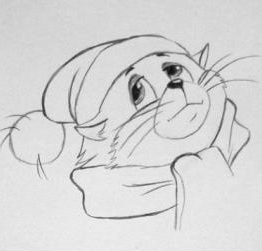
\includegraphics[width=0.42\linewidth]{picture_cat}}
	\hfill
	\subbottom[результат адаптации\label{fig:cat_mesh}]{%
		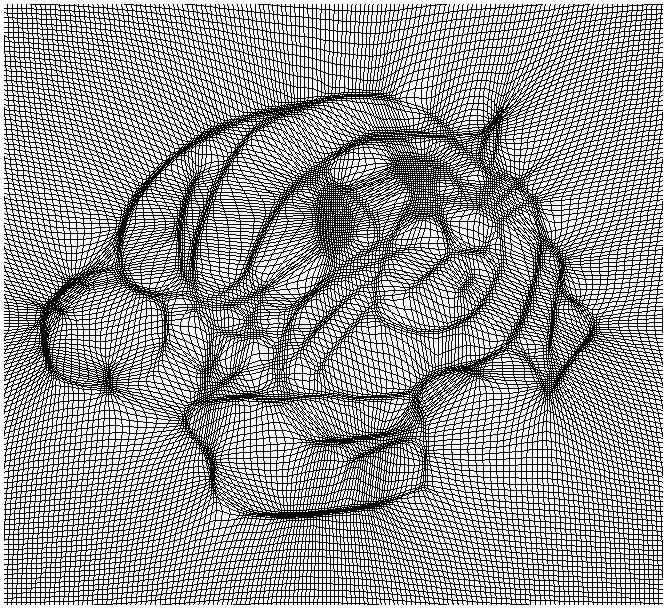
\includegraphics[width=0.45\linewidth]{cat_mesh1}}
}
\caption{Стационарная адаптация сетки путем перераспеделения узлов у произвольно заданной функции сеточной плотности. (a) заданная функция сеточной плотности $\rho$, (б) результат адаптации к заданной функции $\rho$.}
\label{fig:matroskin}
\end{figure}           % Глава 2
\chapter{Численные результаты} \label{ch:ch3}

Применение сеточной адаптации с использованием методики погруженных границ рассматривалось на примере решения двумерной модельной задачи – численного моделирования течения вокруг цилиндрического препятствия при его движении справа налево с дозвуковой скоростью  , соответствующей числу Маха равному 0.2. Число Рейнольдса   рассчитанное по диаметру и скорости движения цилиндра полагалась равным 200. При численном решении данной задачи в качестве характерной скорости выбиралась скорость звука в невозмущенном потоке газа при нормальных условиях. Безразмерный радиус цилиндра   устанавливался равным величине 0.2. Тогда эффективное числа Рейнольдса   при котором проводились расчёты имело значение 400.

Рисунок 1: Фрагменты расчётной подробной сетки 1: слева – зона движения цилиндра, справа – окрестность препятствия.


Рисунок 2: Фрагменты расчётной сетки 2: слева – зона движения цилиндра, справа – окрестность препятствия.

Для проведения расчёта движения цилиндра необходимо иметь подробную сетку на всём пути движения цилиндра, во-первых, для корректного описания физических процессов, происходящих при обтекании препятствия, и во-вторых, для более точного описания границы обтекаемого препятствия при использовании метода погруженных границ. Поэтому использование неподвижных (неадаптивных сеток) приводит к резкому возрастанию вычислительной сложности решения такого типа задач. Применение адаптивной сетки, сгущающейся к границе движущегося тела, и обеспечивающее нужное разрешение сетки в следе за телом, должно уменьшить размер сетки, и, как следствие вычислительную стоимость решения. Таким образом, необходимо сравнить качество численного решения, полученного на трёх сетках – подробной, грубой и грубой с адаптацией.
Для этого расчёты проводились на трёх неструктурированных треугольных сетках. Первая сетка (сетка 1) – подробная сетка с числом узлов равным 391628 (Рис. 1), вторая сетка (сетка 2) – сетка с числом узлов 110372, приблизительно в 3.5 раза меньшим, чем у подробной сетки (Рис. 2). Третья сетка (сетка 3) это сетка 2 адаптирующаяся к поверхности движущегося цилиндрического препятствия и не меняющая своей топологии. На рисунках 3 и 4 показаны фрагменты адаптивной сетки на различные моменты времени положения движущегося цилиндра. Заметим, что в области движения цилиндра для сеток 1 и 2 определен регион квазиравномерной сетки с шагом h  и от него происходит огрубление сетки к границам расчётной области (см. рисунок 3 слева вверху)


Рисунок 3: Сетка 2 – недеформированная (слева вверху) и её адаптация на три момента времени: начало периода  , полтора периода   и два периода  .



Рисунок 4: 	Сетка вблизи препятствия на начало периода   и четыре с половиной периода  

Закон адаптации сетки определяется управляющей функцией   в уравнении (15). Так как обтекаемое тело симметрично, то достаточно определить зависимость управляющей функции только от радиального направления   с центром, совпадающим с центром цилиндра. Данная функция должна определять сгущение точек с внешней и внутренней стороны границы цилиндра и не изменять исходную сетку при удалении от центра цилиндрического препятствия. Этим условиям удовлетворяют функции типа гауссиана с управляющими параметрами

(16)
Здесь амплитуда   и чётные показатели степени  ,   определяют величину сгущения, значения полуширины гауссиана  ,   задают толщины областей сгущение внутри и вне цилиндра, соответственно. В настоящем расчёте эти параметры полагались равными следующим значениям
,  ,  ,  .	(17)
Функция (16) с параметрами (17) трижды непрерывно дифференцируема и её график приведён на рисунке 5.


Рисунок5: График управляющей функции  .

Из этого графика можно видеть, что наиболее сильная адаптация сетки (уменьшение амплитуды A на 46\%) к границе цилиндра наблюдается на расстоянии приблизительно равным   от границы цилиндра во внутренней области и на расстоянии   во внешней области. На расстояниях больших   управляющая функция экспоненциально понижается до единицы, что исключает адаптацию сетки вдали от центра цилиндра в направлении движения цилиндра. Такое изменение сетки можно наблюдать на рисунке 3. Из распределения узлов сетки, показанных на рисунке 3 видно, что в направлении перпендикулярном движению сетка сильно деформируется. Это явление связано с тем, что число узлов в адаптивной сетке не увеличивается, а в направлении перпендикулярном движению исходная недеформированная сетка 2 (слева вверху на рисунке 3) имеет меньшую плотность распределения узлов.
Из рисунков 3 и 4 видно, что адаптация сетки происходит практически однородно и не зависит от положения цилиндра в абсолютной системе координат. То есть фактически можно считать, что деформированная в начальный момент времени сетка перемещается как жёсткая конструкция в направлении движения цилиндра.
Также обратим внимание (см. рисунок 4), что при использовании изотропной управляющей функции (зависимость только от радиуса) не приводит к сильной деформации элементов сетки в области движения цилиндрического препятствия и сетка вне узкой окрестности вдоль границы цилиндра близка к квазиравномерной.
В процессе адаптации грубой сетки 2 размер элементов сетки в окрестности границы цилиндра имеет размер в среднем в 2.5 раза меньший, чем размер аналогичных элементов подробной сетки 1. Это можно видеть на рисунке 6, где показано распределение минимальных высот треугольников на подробной сетке (слева) и на грубой сетке после адаптации (сетка 3). 


Рисунок 6: 	Распределения минимальных высот треугольников в расчётных сетках: по-дробная сетка (слева), адаптированная грубая сетка (справа)

При выполнении расчётов движущегося цилиндра на всех трёх сетках шаг интегрирования по времени выбирался согласно следующему критерию
, 
где   – шаг определяемый устойчивостью разностной схемы и обеспечивающий корректность нестационарного интегрирования,   – временной шаг, выбираемый из условия прохождения приграничных ячеек границей цилиндра не менее чем за один шаг при расчёте временного слоя   
.
Здесь   минимальный размер приграничного элемента сетки на время  .



Рисунок 7: 	Распределение завихренности на четыре момента времени: начало периода  , полто-ра периода  , два периода  и четыре с половиной периода  


Общая картина течения после выполнения расчёта с использованием адаптивной сетки показана на рисунке 7, где приведены поля завихренности на различные моменты времени. В табл.1 приведены средние значение коэффициента сопротивления  и числа Струхаля Sh, полученные по результатам этих расчетов на трёх сетках и экспериментальные значения из работы [34]. Число Струхаля   определено с помощью преобразования Фурье

%	Таблица 1.	Средние значения коэффициентов силы сопротивления и число Струхаля, полученные расчётом на разных сетках. 

%	Эксперимент [34]	Сетка 1	Сетка 2	Сетка 3
%	Sh	0.19	0.189	0.186	0.191
%	
%	1.34	1.218	1.118	1.301
\clearpage           % Глава 3
\chapter*{Заключение}                       % Заголовок
\addcontentsline{toc}{chapter}{Заключение}  % Добавляем его в оглавление
В работе разработан упрощенный быстрый алгоритм динамической адаптации сетки на основе перераспределения узлов с сохранением сеточной топологии. Этот метод в комплексе с методом погруженных границ для описания твёрдых объектов в односвязной области позволяет  эффективное численное исследование движущихся в турбулентных потоках тел.  Помимо использования алгоритма адаптации совместно в погруженными граничными условиями, его можно успешно использоваться для решения задач с «традиционным» описанием подвижных тел граничными сеточными узлами при условии не столь
больших отклонений от их исходного положения (например, разного рода 
колебательных движений), а также для адаптации сетки к полям решения.

Основные результаты работы заключаются в следующем:
%% Согласно ГОСТ Р 7.0.11-2011:
%% 5.3.3 В заключении диссертации излагают итоги выполненного исследования, рекомендации, перспективы дальнейшей разработки темы.
%% 9.2.3 В заключении автореферата диссертации излагают итоги данного исследования, рекомендации и перспективы дальнейшей разработки темы.
\begin{enumerate}
	\item На основе анализа существующих методов динамической сеточной адаптации выбран метод адаптации с движением узлов без изменения топологии сетки.
	\item  Алгоритма динамической адаптации неструктурированной сетки разработан для  использования совместно в методом погруженных граничных условий и функции линий уровня, описывающей геометрию твёрдого тела.
	\item Алгоритм реализаван в рамках некоммерческого исследовательского комплекса программ NOISEtte++, разрабатываемом в отделе вычислительной аэродинамики и аэроакустики ИПМ РАН.
	\item Рассмотренна двумерная постановка для треугольных сеток. Проведен численный расчет задаче о моделировании течения за движущимся цилиндром.
\end{enumerate}


К настоящему времени данная технология разработана применительно к решению двумерных задач газовой динамики на треугольных сетках. Результаты, подтверждающие ее эффективность, продемонстрированны на модельных задачах и, в частности, на задаче о моделировании течения за движущимся цилиндром.

В дальнейшем планируется использовать уравнение движения сетки в полной формулировке, а также обобщение разработанной технологии на трёхмерные постановки. Также предполагается работа по усовершенствованию техники адаптации неструктурированной сетки за счёт улучшения качества адаптивной сетки вблизи погруженной границы обтекаемого тела. 

%% Согласно ГОСТ Р 7.0.11-2011:
%% 5.3.3 В заключении диссертации излагают итоги выполненного исследования, рекомендации, перспективы дальнейшей разработки темы.
%% 9.2.3 В заключении автореферата диссертации излагают итоги данного исследования, рекомендации и перспективы дальнейшей разработки темы.
%% Поэтому имеет смысл сделать эту часть общей и загрузить из одного файла в автореферат и в диссертацию:


В заключение автор
выражает благодарность и большую признательность научному руководителю
Козубской~Т.\:К. за поддержку, помощь, обсуждение результатов и научное
руководство. Также автор благодарит Бахвалова~П.\:А. и~Абалакина~И.\:В.
за помощь в~работе и~обсуждение результатов.
      % Заключение
%\include{Dissertation/acronyms}        % Список сокращений и условных обозначений
%\include{Dissertation/dictionary}      % Словарь терминов
\include{Dissertation/references}      % Список литературы
\include{Dissertation/lists}           % Списки таблиц и изображений (иллюстративный материал)

%%% Настройки для приложений
\appendix
% Оформление заголовков приложений ближе к ГОСТ:
\setlength{\midchapskip}{20pt}
\renewcommand*{\afterchapternum}{\par\nobreak\vskip \midchapskip}
\renewcommand\thechapter{\Asbuk{chapter}} % Чтобы приложения русскими буквами нумеровались

%\chapter{Математическое описание аэродинамики движущихся тел на основе метода погруженных границ на подвижной сетке} \label{app:A}
Для описания движущихся тел в качестве наиболее удобного подхода все большее распространение приобретают методы погруженных границ (в англоязычной научной литературе – Immersed Boundary Conditions или IBC метод)~\cite{mittal2005immersed, boiron2009high, brown2014characteristic}.
Методы погруженных границ составляют целый класс методов, позволяющих обеспечить выполнение граничных условий на поверхности обтекаемых тел в процессе численного расчёта без описания ее геометрии сеточными узлами. Это означает, что может быть использована «сплошная» расчётная сетка, покрывающая всю область определения задачи, включая препятствие. 

Взаимодействие твёрдого тела и окружающей среды при этом может моделироваться несколькими способами. Один из них – это модификация дискретизированных газодинамических уравнений, основанная на геометрическом анализе пространственного расположения используемого разностного шаблона относительно границы твёрдого тела. Другой способ заключается во введении штрафных функций непосредственно в исходные уравнения. Они добавляются в виде источниковых членов и имеют ненулевое значение только в узлах расчётной сетки, находящихся внутри твёрдого тела.

Применение погруженных граничных условий заметно упрощает воспроизведение движения тел даже, если они имеют сложную геометрическую форму. Так, при использовании штрафных функций, изменение пространственного положения обтекаемого тела на каждом временном шаге сводится лишь к изменению источниковых членов в решаемых уравнениях, а не к ресурсоемкому перестроению расчётной сетки, требуемому при описании границы сеточными узлами.

\section{Математическая модель для неподвижных сеток} \label{app:A1}
Следуя методу Бринкмана штрафных функций, система уравнений Навье-Стокса, описывающая течение в области $\Omega_f$ вокруг твёрдого тела $\Omega_B$ с границей $\partial \Omega_B$ , модифицируется следующим образом~\cite{mittal2005immersed, boiron2009high}:
\begin{equation}
\left\{
\begin{aligned}
&\mathbf{Q}_t + \nabla \cdot \mathbf{F}(\mathbf{Q})+S_{\eta} = \nabla\cdot\mathbf{F}_{\nu}(\nabla \mathbf{Q}), \quad (\mathbf{x}, t) \in \Omega_f \cup \Omega_B \cup \partial\Omega_B\\
&\mathbf{Q}(t=0) = \mathbf{Q}_0(\mathbf{x})\\
&S_{\eta} = \eta^{-1} \chi (0, \rho(\mathbf{u} -\mathbf{U}_B), E)
\end{aligned}
\right. ,
\label{eq:NS}
\end{equation}
где   $\mathbf{Q} = (\rho, \rho\mathbf{u}, E)$ – вектор безразмерных консервативных переменных,  $\mathbf{F}$ и  $\mathbf{F}_{\nu}$ – конвективные и вязкие потоки, $\rho$ – плотность газа,  $\mathbf{u}$ – вектор скорости, $\mathbf{U}_B$   – скорость движения твёрдого тела,  $E$ – полная энергия. Система замыкается уравнением состояния идеального газа: $p = (\gamma - 1)\rho \varepsilon$, где $\varepsilon$  – внутренняя энергия, $\gamma = 1.4$  – показатель адиабаты, а полная энергия определяется соотношением:  $E = \rho \varepsilon + \rho\mathbf{u}^2/2$.

Характеристическая функция $\chi$ определяет геометрическое место обтекаемого тела:
\begin{equation}
\chi = \left\{
\begin{aligned}
&1, \quad \mathbf{x}\in \overline{\Omega}_B\\
&0, \quad \mathbf{x}\in \Omega_f
\end{aligned}
\right. .
\label{eq:chi}
\end{equation}

Как видно из~\eqref{eq:NS}, источниковые члены $S_\eta$, называемые штрафными функциями, добавляются только в уравнения импульса и энергии. В точках сетки, где характеристическая функция  $\chi\ne0$ (т.е. внутри препятствия), система трансформируется в модель Бринкмана пористой среды с параметром $\eta$, определяющим ее проницаемость: $0<\eta<<1$: чем меньше коэффициент $\eta$, тем точнее воспроизводятся граничные условия при  $\mathbf{x}\in\partial\Omega_B$.

В работе~\cite{abalakin2015} возможности данного метода были продемонстрированы на примере решения двумерных модельных задач по расчёту дозвукового и сверхзвукового течения вокруг цилиндра.  Работа~\cite{abalakin2018} демонстрирует численное решение задачи турбулентного обтекания трёхмерного цилиндра.
Для численного решения системы уравнений~\eqref{eq:NS} использовалась оригинальная EBR (Edge-Based Reconstruction) схема повышенной точности, основанная на квазиодномерной рёберно-ориентированной реконструкции переменных~\cite{abalakin2016edge}.
\section{Математическая модель для подвижных сеток}
Для описания течения на движущихся адаптивных (деформируемых) сетках использовался смешанный эйлерово-лагранжев (СЭЛ) подход~\cite{hirt1974arbitrary, golovizin1981} использования уравнений газовой динамики, как законов сохранения. Этот подход можно интерпретировать как промежуточное описание движения сплошной среды между эйлеровым подходом, использующим абсолютную систему координат и лагранжевым описанием, использующим систему координат, связанную с локальной скоростью движения среды. То есть выбирается такая система координат, которая не фиксирована по времени и не перемещается со скоростью среды. 

Рассмотрим систему координат, движущуюся со скоростью $\dot{\mathbf{x}}$, равной скорости деформации сетки $\mathbf{U}_M$. Рассмотрим интеграл от вектора консервативных производных по произвольному жидкому объёму $V(t)$. Тогда полная производная от жидкого объёма запишется следующим образом~\cite{budak2002}, с.259]
\begin{equation}\label{eq:integral_derivative}
\frac{d}{dt}\int \limits_{V(t)}\mathbf{Q}dV = \int \limits_{V(t)}\left[\mathbf{Q}_t + \nabla \cdot (\mathbf{Q}\dot{\mathbf{x}})\right]dV .
\end{equation}
Из законов сохранения~\eqref{eq:NS} следует, что $\mathbf{Q}_t = -\nabla \cdot \mathbf{F}(\mathbf{Q})-S_{\eta} + \nabla\cdot\mathbf{F}_{\nu}(\nabla \mathbf{Q})$. Подставляя частную производную по времени в~\eqref{eq:integral_derivative} получаем систему законов сохранения в СЭЛ форме
\begin{equation}\label{eq:integral_derivative2}
\frac{d}{dt}\int \limits_{V(t)}\mathbf{Q}dV = 
-\int \limits_{V(t)}\left[ \nabla \cdot(\mathbf{F} - \mathbf{Q}\dot{\mathbf{x}}) - \nabla\cdot\mathbf{F}_{\nu}(\nabla \mathbf{Q}) + S_{\eta} \right] dV .
\end{equation}
При заданном законе движения сетки  $\dot{\mathbf{x}} = \mathbf{U}_M$ система законов сохранения~\eqref{eq:integral_derivative2} определяет математическую модель необходимую для проведения расчётов на адаптивной сетке с использованием метода погруженных границ. Заметим, что при  $\dot{\mathbf{x}} = 0$ система~\eqref{eq:integral_derivative2} имеет эйлеровскую форму представления законов сохранения, а при $\dot{\mathbf{x}} = \mathbf{u}$  – систему законов сохранения в лагранжевой форме.
\section{Технология расчета системы газодинамических уравнений в СЭЛ форме на движущихся сетках с неизменной топологией для треугольной сетки}
Кратко разработанную технологию можно представить для решения системы~\eqref{eq:integral_derivative2} следующим образом. Для простоты дальнейших выкладок определим вязко-невязкий поток  $\mathbf{F(Q, \nabla Q)} \equiv \mathbf{F(Q)} - \mathbf{F}_{\nu}( \nabla \mathbf{Q})$  и положим равным нулю источниковый член (для дальнейших выкладок он не имеет принципиального значения). Для аппроксимации системы законов сохранения~\eqref{eq:integral_derivative2} будем использовать конечно-объёмный подход, который в равной степени применим как к статическим сеткам, так и к меняющимся по любому непрерывному закону. Определим переменные в узлах неструктурированной сетки и будем рассматривать жидкий контрольный объём $V(t)$  в системе~\eqref{eq:integral_derivative2} как $i$-ую деформируемую сеточную ячейку $K_i(t)$, являющуюся контрольным объёмом, построенным вокруг узла $i$. Тогда для записи конечно-объёмной схемы для системы~\eqref{eq:integral_derivative2} заменим в правой части этой системы интегрирование по объёму интегрированием по поверхности  $\partial K_i(t)$. Получаем
\begin{equation}\label{eq:integral_derivative3}
\frac{d}{dt}\iint \limits_{K_i(t)} \mathbf{Q}dV + 
-\int \limits_{\partial K_i(t)}\mathbf{F(Q, \nabla Q)} \cdot \mathbf{n} \,dS - 
\int \limits_{\partial K_i(t)}\mathbf{Q}(\mathbf{U}_M\cdot \mathbf{n})dS = 0 ,
\end{equation}
где  $\mathbf{n}$ – нормаль к границе ячейки. Таким образом, интегральное уравнение, а, следовательно, и конечно-объёмная разностная схема приобретает дополнительное слагаемое, пропорциональное скорости движения граней сеточных ячеек.

При аппроксимации уравнений Эйлера или Навье-Стокса на движущихся неструктурированных сетках принципиально важным является одновременное обеспечение консервативности (выполнения законов сохранения) и геометрической консервативности (точной передачи однородного потока). Консервативность метода обеспечивается благодаря строгому следованию конечно-объёмному подходу. Для геометрической консервативности  аппроксимация уравнения~\eqref{eq:integral_derivative3} должна быть точной, если  $\mathbf{Q}$ не зависит от координат и времени. Второе слагаемое при этом зануляется, поэтому рассмотрим аппроксимацию третьего слагаемого. Она осуществляется по-разному при применении явных и неявных схем для интегрирования разностного уравнения~\eqref{eq:integral_derivative3}.

В случае многостадийной явной схемы (схемы Рунге-Кутта) необходимо на каждом временном подслое аппроксимировать последнее слагаемое в \eqref{eq:integral_derivative3} так, чтобы при $\mathbf{Q} = const$  аппроксимация оказывалась точной. Для этого будем использовать следующую аппроксимацию на грани двух контрольных объёмов с центрами в точках $R$ и $L$ $(\partial K_L(t)\cap\partial K_R(t) )$:
\begin{equation}\label{eq:approx}
\int \limits_{\partial K_i(t)}\mathbf{Q}(\mathbf{U}_M\cdot \mathbf{n})dS \approx \frac{\mathbf{Q}_L + \mathbf{Q}_R}{2} \int \limits_{\partial K_L(t)\cap\partial K_R(t)} \mathbf{U}_M\cdot \mathbf{n}\,dS,
\end{equation}
а оставшийся интеграл в правой части считать точно на каждый момент времени. В разработанной технологии в течение одного временного шага скорость движения сеточных узлов предполагается постоянной. Если $K_i(t)$  есть барицентрический\footnote{Под барицентрическим контрольным объёмом для треугольной сетки понимается многогранник, границей которого, является ломаная соединяющая центры рёбер и центры тяжести треугольников.}  контрольный объём, то радиус-вектор каждой вершины этого объёма является линейной комбинацией радиус-векторов сеточных узлов. В результате средняя скорость по каждой грани сеточной ячейки также является постоянной в пределах шага, а интеграл в правой части \eqref{eq:integral_derivative3} за счёт изменения площадей граней – линейной функцией времени. Величины контрольных объёмов, следовательно, являются квадратичной функцией. Поэтому, чтобы выполнялась геометрическая консервативность в \eqref{eq:integral_derivative3}, необходимо использовать метод Рунге-Кутта не ниже 2-го порядка.

Для записи неявного метода Эйлера проинтегрируем \eqref{eq:integral_derivative3} по времени. Получаем
\begin{equation}\label{eq:integral_time}
\iint \limits_{K_i(t^{n+1})} \mathbf{Q}dV  - \iint \limits_{K_i(t^{n})} \mathbf{Q}dV+ 
\int \limits_{t^n}^{t^{n+1}} \int \limits_{\partial K_i(t)}\mathbf{F(Q, \nabla Q)} \cdot \mathbf{n} \,dS - 
\int \limits_{t^n}^{t^{n+1}} \int \limits_{\partial K_i(t)}\mathbf{Q}(\mathbf{U}_M\cdot \mathbf{n})dS = 0 ,
\end{equation}
Чтобы аппроксимация была точной при  $\mathbf{Q} = const$, запишем для третьего слагаемого в \eqref{eq:integral_derivative3} аппроксимацию
\begin{equation}\label{eq:approx_time}
\int \limits_{t^n}^{t^{n+1}} \int \limits_{\partial K_i(t)}\mathbf{Q}(\mathbf{U}_M\cdot \mathbf{n})dS \approx \frac{\mathbf{Q}^{n+1}_L + \mathbf{Q}^{n+1}_R}{2} \int \limits_{t^n}^{t^{n+1}} \int \limits_{\partial K_L(t)\cap\partial K_R(t)} \mathbf{U}_M\cdot \mathbf{n}\,dS.
\end{equation}
Интеграл в правой части также вычисляется аналитически.

Аппроксимация второго слагаемого в \eqref{eq:integral_derivative3} для конвективной части системы уравнений Навье-Стокса осуществляется при помощи схем с квазиодномерной реконструкцией переменных, как и в случае недеформируемой сетки. Они основаны на том, что повышение порядка точности осуществляется посредством квазиодномерной рёберно-ориентированной реконструкции значений физических переменных в центр ребра ~\cite{abalakin2016edge}. Коэффициенты реконструкции можно брать с недеформированной сетки или пересчитывать на каждом временном слое. 

Аппроксимация вязких членов в уравнении Навье-Стокса проводится методом Галёркина на основе полиномов 1-го порядка как в случае покоящейся, так и в случае движущейся сетки и не требует внесения изменений. 




        % Приложения

\end{document}
